\chapter{The Lip Reed}\label{ch:lipreed}
The dynamics of wind instruments can be modelled by acoustic tubes as presented in Chapter 5. Excitation of these instruments happens either by blowing a jet of air across an opening, such as in a flute, or by the buzzing of a \textit{reed}. In \cite{Fletcher1998}, the authors state that all wind-instrument reeds fall into one of three categories: the single reed, (clarinet, saxophone), the double reed (oboe, bassoon) and the lip reed (trumpet, trombone). The latter will be the focus of this chapter.

% Brass instruments are excited by the lips of the player. The opening and closing of the lips causes a vibration
Sections \ref{sec:webstersExcitation} and \ref{sec:pulseTrain} presented a physically inspired pulse train that attempts to model the opening and closing of the lips, using a clipped sinusoidal signal. A more physical approach, which is bidirectional, is to model the lips as a mass-spring-damper system that interacts with the left boundary of the tube. The literature describes lip reed models with varying degrees of freedom (DoF) (see \cite{Fletcher1998,Harrison2018} for an overview). Recent work includes vortex-induced vibration into the lip reed model, that allows for the buzzing of the lips without the need of an acoustic tube [\hyperref[ch:listOfPublications]{S1}]. 

As the contribution of this project to a brass instrument model was mainly focused on the resonator, the simple `outward striking door model' was chosen, which is a simple single one-DoF mass-spring-damper system. The model is as presented in \cite{Bilbao2009Reed} excluding the collision. An alternative collision model was added in paper \citeP[H] and will be elaborated on in Chapter \ref{ch:trombone}.

This chapter starts by introducing the mass-spring-damper system, after which the lip reed model will be given in continuous and discrete time. The lip reed will be coupled to the first-order system of equations presented in \ref{sec:firstOrderSystem}. Unless denoted otherwise, this chapter follows \cite{Harrison2018}. 

\section{Mass-spring systems revisited: Damping}\label{sec:massSpringDamping}
Before moving on to the lip reed system, the mass-spring system given in Section \ref{sec:massSpringSystem} will be extended to contain damping. 

Recall the mass spring system presented in Eq. \eqref{eq:massSpringPDE}, where $u=u(t)$ is the displacement of the mass from its equilibrium position (in m). Damping can be easily be added to yield a mass-spring-damper system as follows:
\begin{equation}\label{eq:massSpringDampingPDE}
    M\ddot u = -Ku - R\dot u,
\end{equation}
with mass $M$ (in kg), spring constant $K$ (in N/m) and damping coefficient $R$ (in kg/s). Figure \ref{fig:massSpringDamper} shows the behaviour of the system for different values of $R$. 

Equation \eqref{eq:massSpringDampingPDE} can then be discretised to the following FD scheme:
\begin{equation}\label{eq:massSpringDampingFDS}
    M\dtt \un = -K\un - R\dtd \un.
\end{equation}
Expanding and solving for $u^{n+1}$ yields the following update equation:
\begin{equation}\label{eq:massSpringDampingUpdate}
    \left(1+\frac{Rk}{2M}\right)u^{n+1} = 2 \un - u^{n-1} - \frac{Kk^2}{M}\un + \frac{Rk}{2M}u^{n-1}.
\end{equation}

\def\figWidth{0.32}
\begin{figure}[h]
    \centering
    \subfloat[$R=0$.\label{fig:massSpringDamper1}]{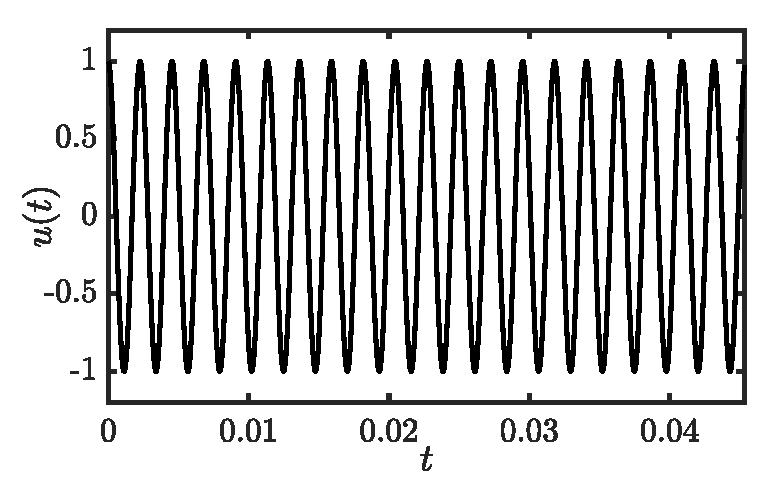
\includegraphics[width=\figWidth\textwidth]{figures/exciters/lipreed/massSpringDamper1.eps}}\hfill
    \subfloat[$R=50$.\label{fig:massSpringDamper2}]{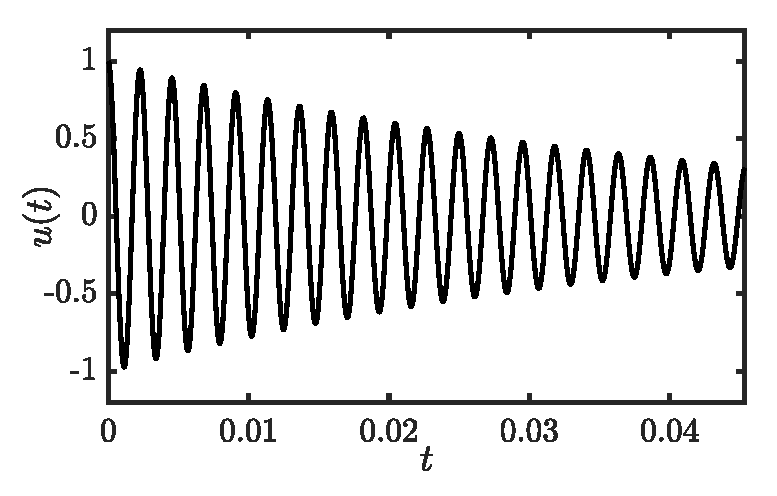
\includegraphics[width=\figWidth\textwidth]{figures/exciters/lipreed/massSpringDamper2.eps}}\hfill
    \subfloat[$R=200$.\label{fig:massSpringDamper3}]{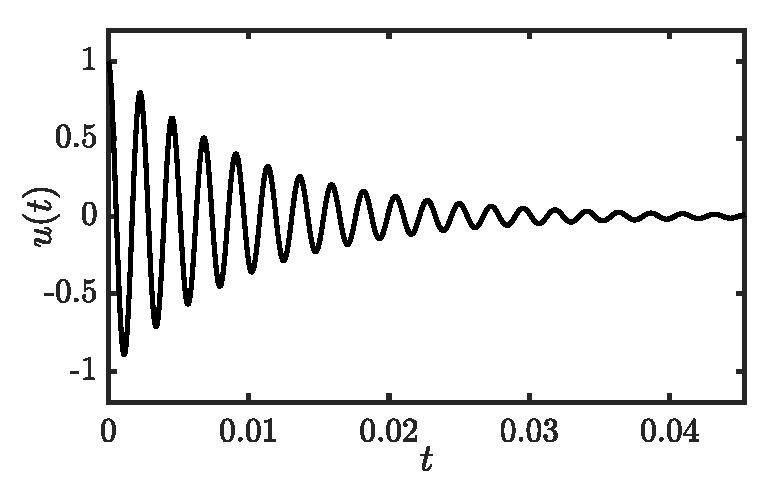
\includegraphics[width=\figWidth\textwidth]{figures/exciters/lipreed/massSpringDamper3.eps}}
    \caption{The mass-spring-damper system in Eq. \eqref{eq:massSpringDampingPDE} with $f_0=440$ Hz for different values of $R$. \label{fig:massSpringDamper}}
\end{figure}

\subsection{Energy analysis}
Following Section \ref{sec:energyAnalysis} (without explicitly following the steps for brevity), one can obtain the energy of Eq. \eqref{eq:massSpringDampingFDS} through a multiplication of the scheme by $(\dtd \un)$ to get
\begin{equation}\label{eq:massSpringDampingPreEnergyBalance}
    M(\dtt \un)(\dtd \un) = -K(\dtd \un)\un - R(\dtd \un)^2.
\end{equation}
As there is damping present in the system, the energy balance will be of the form 
\begin{equation*}
    \dtp \h = -\q.
\end{equation*}
Using identities \eqref{eq:prodIdentity1} and \eqref{eq:prodIdentity2}, $\h$ and $\q$ can be obtained from Eq. \eqref{eq:massSpringDampingPreEnergyBalance} 
\begin{equation}\label{eq:energyBalanceMassSpringDamper}
    \h = \t + \v, \qwiq
    \t = \frac{M}{2}(\dtm\un)^2, \qaq \v = \frac{K}{2}\un e_{t-}\un,
\end{equation} 
and
\begin{equation}\label{eq:massDampingEnergy}
    \q = R(\dtd \un)^2.
\end{equation}

Figure \ref{fig:massSpringDamperEnergy} shows the energy output of the mass spring damper system with $R = 50$ and $f_0 = 2\pi\sqrt{K/M} = 440$ Hz. One can observe that the damping term causes the system to lose energy when the mass is in motion (high kinetic energy).
\begin{figure}[h]
    \centering
    \begin{tikzpicture}[->,node distance=3cm,
        thick,main node/.style={circle,draw}]
    
        \node[] (image) at (0,0) {
        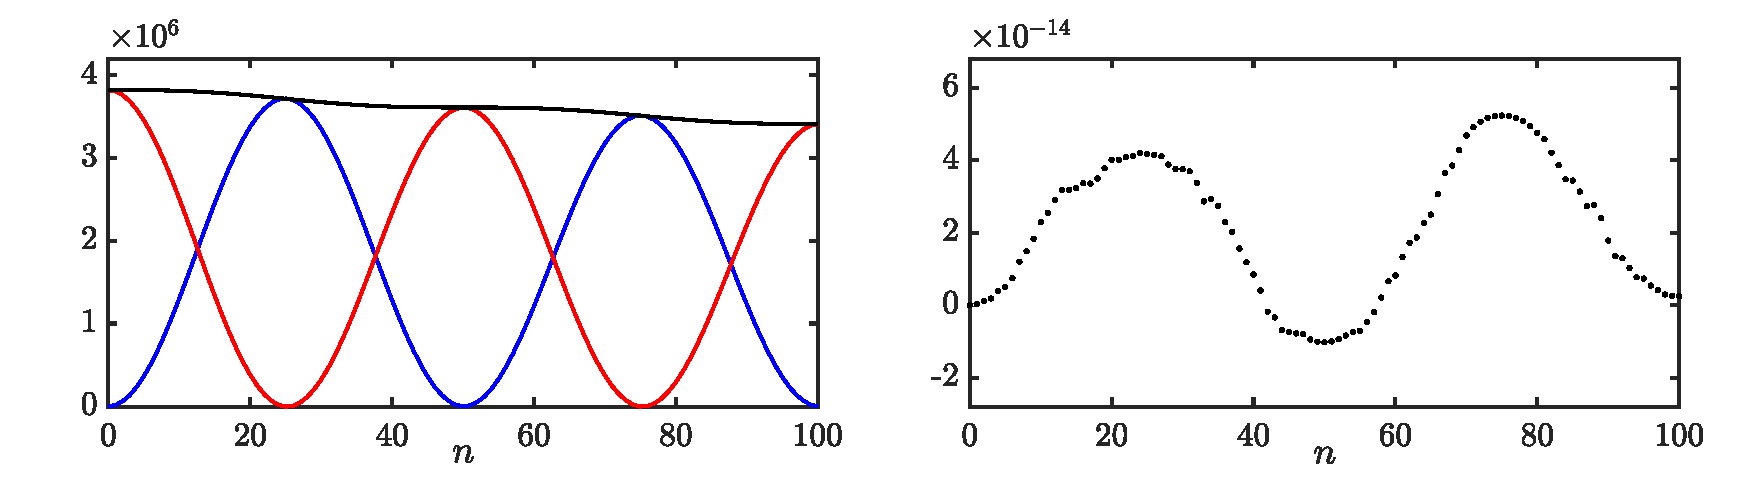
\includegraphics[width=\textwidth]{figures/exciters/lipreed/massSpringDamperEnergy.eps}
        };
    
        \node[] (he) at (0.2,0.5) {\small $\mathfrak{h}_\text{e}$};

        \node[] (h) at (-5.8, 1) {\small $\mathfrak{h}$};
        \node[] (v) at (-5.8, 0.5) {\small $\color{red}\mathfrak{v}$};
        \node[] (t) at (-5.8, 0) {\small $\color{blue}\mathfrak{t}$};
      \end{tikzpicture}
      \caption{The potential (red), kinetic (blue), and total (black) energy of the mass-spring-damper system. The right panel shows the normalised energy (according to Eq. \eqref{eq:normalisedEnergyDamping}) and shows that the deviation of the energy is within machine precision. \label{fig:massSpringDamperEnergy}}
\end{figure}

\section{Continuous time}\label{sec:lipreedContinuous}
As mentioned at the beginning of this chapter, the lip reed will be modelled as a mass-spring-damper system as in Eq. \eqref{eq:massSpringDampingPDE}. The system will be coupled to an acoustic tube described by the first-order system of PDEs described in Section \ref{sec:firstOrderSystem}, Eq. \eqref{eq:firstOrderSystem}.
% :
% \begin{subequations}\label{eq:firstOrderSystemLipReedCh}
%     \begin{align}
%         \frac{S}{\rho_0 c^2}\partial_t p &= -\partial_x(Sv),\label{eq:contPressureLipReedCh}\\
%         \rho_0\partial_tv &= -\partial_xp\label{eq:discVelocityLipReedCh},
%     \end{align}
% \end{subequations} %An additional term  due to the pressure difference between the mouth and the tube is added to the equation and t

Using dots to denote derivatives with respect to time $t$, the PDE of the lip reed connected to an acoustic tube is defined as
\begin{equation}\label{eq:lipReedDimensional}
    M\ddot y = -K y - R \dot y + S_\text{r}\Delta p,
\end{equation}
with displacement of the lip reed from equilibrium $y = y(t)$ (in m), mass of the lip reed $M > 0$ (in kg), lip stiffness $K\geq 0$ (in N/m), damping coefficient $R\geq 0$ (in kg/s), and effective surface area of the lip $S_\text{r}\geq 0$ (in m$^2$). Furthermore,  
\begin{equation}\label{eq:deltaP}
    \Delta p = \Delta p(t) = P_\text{m} - p(0,t)
\end{equation}
is the difference between the pressure in the mouth $P_\text{m} = P_\text{m}(t)$ and the pressure at the left boundary of the acoustic tube $p(0,t)$ (all in Pa). The acoustic tube can be described by the first-order system presented in Section \ref{sec:firstOrderSystem}. See Figure \ref{fig:lipSystem} for a schematic representation of the lip reed.
\begin{figure}[t]
    \centering
    \begin{tikzpicture}
    
    \def\radius{6}; % Radius of the string (>2!)
    \pgfmathsetmacro{\reps}{3}; % How may back-and-forths in the drawing of the springs
    \def\bowSpacing{0.2};
    \def\drawingSpacing{1.5}
    \def\bowWidth{5};
    
    \def\woodWidth{1}; %>0.3
    \def\massWidth{2};
    \def\bridgeHeight{3};
    \def\bridgeWidth{4};
    \def\cornerRadius{0.15};
    \def\stringWidth{0.2};
    \pgfmathsetmacro{\tinyRadius}{\stringWidth*0.1};
    \pgfmathsetmacro{\stringWidthMinTinyRad}{((\stringWidth-(2*\tinyRadius)))*0.5};
    
    % draw airflow
    
    %draw airflow
    \def\rightAirFlow{0}; % have the right airflow bulge (1) or not (0)
    \foreach \idx in {1,...,5}
    {
        \pgfmathsetmacro{\scaleLeft}{0.5 - 0.1 * \idx};
        \ifnum\rightAirFlow=1
            \pgfmathsetmacro{\scaleRight}{0.5 - 0.1 * \idx};
        \else
            \pgfmathsetmacro{\scaleRight}{0};
        \fi
        \begin{scope}[decoration={
            markings,
            mark=between positions 0.15 and 0.85 step 0.35
         with {\arrow{>}}}
            ]
        % \node at (0, \idx) {\scale};
         \draw [gray!40, 
         xshift=-2.5cm, 
         yshift= -\idx * 0.3cm, 
         dotted, 
         line width=0.3mm, postaction={decorate}] plot [smooth, tension = 0.5] coordinates { (0,1*\scaleLeft) (1,0.75*\scaleLeft) (2,0) (4, 0) (5, 0.75*\scaleRight) (6,1*\scaleRight)} ;
         \end{scope}
    }
    % \def\scale{0.5};
    % \draw [gray, xshift=-2.5cm, yshift=-0cm] plot [smooth, tension = 0.5] coordinates { (0,1*\scale) (1,0.75*\scale) (2,0) (4, 0) (5, 0.75*\scale) (6,1*\scale)};
    % \def\scale{0.25};
    % \draw [gray, xshift=-2.5cm, yshift=-1.2cm] plot [smooth, tension = 0.5] coordinates { (0,1*\scale) (1,0.75*\scale) (2,0) (4, 0) (5, 0.75*\scale) (6,1*\scale)};
    % \def\scale{0};
    % \draw [gray, xshift=-2.5cm, yshift=-1.5cm] plot [smooth, tension = 0.5] coordinates { (0,1*\scale) (1,0.75*\scale) (2,0) (4, 0) (5, 0.75*\scale) (6,1*\scale)};
    
    \node (r0) at ( 1.0,  -0.5 ) {}; % root
    \node (s0) at ( 1.0, 0.1 ) {}; % extreme
    \node (s1) at ( 1.6, 0.1 ) {}; % extreme

    % DRAW TREE
    \fill[fill=white] (r0.center)--(s0.center)--(s1.center);
    
    % \draw plot [smooth] coordinates {(-3, -3) (-2, 2) (-1, -3};
    \node at (0,0) [rectangle,draw, fill = white, minimum height=1cm,minimum width= \massWidth cm] (Mr) {$M$};
    %top
    % \draw[-] (-3, 2) -- (3, 2) node[below, midway] (top) {};
    % \draw[-] (-2, 3) -- (4, 3) node[below, midway] (top) {};
    % \draw[-] (-3, 2) -- (-2, 3) node[below, midway] (top) {};
    % \draw[-] (4, 3) -- (3, 2) node[below, midway] (top) {};
    \draw[-] (-2.5, 2.5) -- (3.5, 2.5) node[below, midway] (top) {};
    %bottom
    \draw[-] (-3, -2) -- (3, -2) node[below, midway] (bottom) {};
    \draw[-] (-2, -1) -- (4, -1) node[below, midway] (bottom) {};
    \draw[-] (-3, -2) -- (-2, -1) node[below, midway] (top) {};
    \draw[-] (4, -1) -- (3, -2) node[below, midway] (top) {};

    % draw mass
    
    \draw[-] (-1, 0.5) -- (0, 1.5) node[] (left) {};

    \draw[-] (1, 0.5) -- (2, 1.5) node[] (topRight) {};

    \draw[-] (0, 1.5) -- (2, 1.5) node[] (top) {};

    \draw[-] (2, 1.5) -- (2, 0.5) node[] (right) {};

    \draw[-] (0.5 * \massWidth, -0.5) -- (2, 0.5) node[] (bottomRight) {};

    \node[rotate = 0] at (0.5, 1) (Sr) {$S_\text{r}$};

    \def\xOffset{0.3};
    % draw spring
    \filldraw[black] (-0.5 + \xOffset, 2.5) circle (1pt) node[anchor=center](topSpring){};    
    \draw[-] (-0.5 + \xOffset, 2.5) -- (-0.5 + \xOffset, 2.3);
    \draw[-] (-0.5 + \xOffset, 2.3) -- (-0.75 + \xOffset, 2.2);
    %switched these around because of the color
    \draw[-] (-0.25 + \xOffset, 2.02) -- (-0.75 + \xOffset, 1.84);
    \draw[-] (-0.75 + \xOffset, 2.2) -- (-0.25 + \xOffset, 2.02);
    \draw[-] (-0.75 + \xOffset, 1.84) -- (-0.25 + \xOffset, 1.66);
    \draw[-] (-0.25 + \xOffset, 1.66) -- (-0.75 + \xOffset, 1.52);
    \draw[-] (-0.75 + \xOffset, 1.52) -- (-0.25 + \xOffset, 1.3);
    \draw[-] (-0.25 + \xOffset, 1.3) -- (-0.5 + \xOffset, 1.2);
    \draw[-] (-0.5 + \xOffset, 1.2) -- (-0.5 + \xOffset, 1.0);
    \filldraw[black] (-0.5 + \xOffset, 1.0) circle (1pt) node[anchor=center](bottomSpring){};    
    \node at (-1 + \xOffset, 1.75) (K) {$K$};
    
    \def\dashpotHeight{-0.25}
    % draw dashpot
    \filldraw[black] (1.5 - \xOffset, 2.5) circle (1pt) node[anchor=center](topDashPot){};
    \draw[-] (1.5 - \xOffset, 2.5) -- (1.5 - \xOffset, 1.4 - \dashpotHeight);

    \draw[-] (1.3 - \xOffset, 1.4 - \dashpotHeight) -- (1.7 - \xOffset, 1.4 - \dashpotHeight);

    \draw[-] (1.25 - \xOffset, 1.7 - \dashpotHeight) -- (1.25 - \xOffset, 1.35 - \dashpotHeight);
    \draw[-] (1.75 - \xOffset, 1.35 - \dashpotHeight) -- (1.75 - \xOffset, 1.7 - \dashpotHeight);

    \draw[-] (1.25 - \xOffset, 1.35 - \dashpotHeight) -- (1.75 - \xOffset, 1.35 - \dashpotHeight);
    \draw[-] (1.5 - \xOffset, 1.35 - \dashpotHeight) -- (1.5 - \xOffset, 1.0);

    \filldraw[black] (1.5 - \xOffset, 1.0) circle (1pt) node[anchor=center](bottomDashpot){};    
    \node at (1.0 - \xOffset, 1.75) (sigma) {$R$};
    
    
    % pressure labels
    \def\pressOffset{0.3}
    \def\backgroundOpacity{0.4}
    \node[fill = white, fill opacity=\backgroundOpacity, text opacity = 1] at (-2, -0.6 - \pressOffset) (Pm) {$P_\text{m}(t)$};
    \node[fill = white, fill opacity=\backgroundOpacity, text opacity = 1] at (0.5, -0.8 - \pressOffset) (deltaP) {$\Delta p(t)$};
    \node[fill = white, fill opacity=\backgroundOpacity, text opacity = 1] at (3.2, -0.6 - \pressOffset) (p) {$p(0,t)$};

    
    % y and H0
    \def\axisLineWidth{0.07};
    \draw[dashed, color = gray] (3.65, 0) -- (1.5, 0);
    \node at (4.2, 1.5) {$y(t)$};
    
    \draw[->] (3.75, -1.5) -- (3.75, 1.5);
    \node at (4, 0) {$0$};
    \draw (3.75 - \axisLineWidth, 0) -- (3.75 + \axisLineWidth, 0) {};

    \draw (3.75 - \axisLineWidth, -1.5) -- (3.75 + \axisLineWidth, -1.5) {};
    \node at (4.2, -1.5) {$-H_0$};
    
    % width
    \draw[black!70] (-1, 0.6) -- (1, 0.6) {};
    \draw[black!70] (-1, 0.55) -- (-1, 0.65) {};
    \draw[black!70] (1, 0.55) -- (1, 0.65) {};
    \node at (0, 0.75) (w) {$w$};
% \begin{scope}[very thick,decoration={
%     markings,
%     mark=at position 0.5 with {\arrow{>}}}
%     ] 
%     \draw[postaction={decorate}] (-4,0)--(4,0);
% \end{scope}
    
    \end{tikzpicture}
    \caption{Lip-reed system with parameters as appear in Section \ref{sec:lipreedContinuous}. (Adapted from paper \citeP[H].)}
    \label{fig:lipSystem}
\end{figure}

The pressure difference in Eq. \eqref{eq:deltaP} causes a volume flow velocity (in  m$^3$/s) and follows the Bernoulli equation
\begin{equation}
    U_\text{B} = U_\text{B}(t) = w[y + H_0]_+\text{sgn}(\Delta p) \sqrt{\frac{2|\Delta p|}{\rho_0}},
\end{equation}
with effective lip-reed width $w$ (in m), density of air $\rho_0$ (in kg/m$^3$), static equilibrium separation $H_0$ (in m). Moreover, $[\cdot]_+$ describes the `positive part of' (see Chapter \ref{ch:collisions}). The negative equilibrium separation $-H_0$ can be seen as the location of the lower lip, and when $y + H_0 \leq 0$, the lips are closed and $U_\text{B}$ is 0. Another volume flow (in m$^3$/s) is generated by the lip reed itself according to
\begin{equation}
    U_\text{r} = U_\text{r}(t) = S_\text{r} \dot y,
\end{equation}
and assuming that the volume flow velocity is conserved, the total air volume entering the acoustic tube at the left boundary is defined as
\begin{equation}
    S(0)v(0,t) = U_\text{B}(t) + U_\text{r}(t).
\end{equation} 

\subsubsection{Compact PDE}
To reduce the number of variables in later derivations in this chapter, one can divide all terms in Eq. \eqref{eq:lipReedDimensional} by $M$ to obtain
\begin{equation}
    \ddot y = -\omega_0^2 y - \sigma_\text{r} \dot y + \frac{S_\text{r}}{M}\Delta p,
\end{equation}
with angular frequency of the lip reed $\omega_0 = \sqrt{K/M}$ (in rad/s) and loss parameter $\sigma_\text{r} = R / M$ (in s$^{-1}$). 

\section{Discrete time}\label{sec:discreteLipReed}
\def\nph{}
\def\nphSys{n+1/2}
This section follows the discretisation and derivation given in \cite[Sec. 5.1.3, pp. 140--141]{Harrison2018}, with a slight change in notation.

The variables $y$, $\Delta p$, and thereby $U_\text{B}$ and $U_\text{r}$ are placed on the interleaved temporal grid\footnote{The variables are placed on the non-interleaved spatial grid, as the lip reed interacts with the boundary of the tube ($x=0$).}, and the equations presented above can be discretised to the following system:
\begin{subequations}\label{eq:discreteLipSystem}
    \begin{align}
        \delta_{tt}y^{\nphSys} &= -\omega_0^2\mu_{t\cdot}y^{\nphSys}-\sigma_\text{r}\delta_{t\cdot}y^{\nphSys} + \frac{S_\text{r}}{M}\Delta p^{\nphSys},\label{eq:discReed}\\
        \Delta p^{\nphSys} &= P_\text{m} - \mu_{t+}p_0^n,\label{eq:pDiff}\\
        U_\text{B}^{\nphSys} &= w[y^{\nphSys}+H_0]_+\text{sgn}(\Delta p^{\nphSys})\sqrt{\frac{2|\Delta p^{\nphSys}|}{\rho_0}},\label{eq:bernoulli}\\
        U_\text{r}^{\nphSys} &= S_\text{r}\delta_{t\cdot}y^{\nphSys},\label{eq:Ur}\\
        \mu_{x-}(S_{1/2}v_{1/2}^{\nphSys}) &= U_\text{B}^{\nphSys} + U_\text{r}^{\nphSys}.\label{eq:UbUr}
    \end{align}
\end{subequations}
Here, $p_0^n$ and $S_{1/2}v_{1/2}^{\nphSys}$ are discrete values at the left boundary of an acoustic tube described by system \eqref{eq:firstOrderFDS}. Expanding the operators in Eq. \eqref{eq:discReed} and solving for $y^{n+3/2}$, yields
\begin{equation}\label{eq:updateEqLipreed}
    % \left(1 + \frac{\omega_0^2 k^2}{2} + \frac{\sigma_\text{r} k}{2}\right)y^{n+3/2} &= 2 y^{n+1/2} - \left(1 + \frac{\omega_0^2 k^2}{2} - \frac{\sigma_\text{r} k}{2}\right) y^{n-1/2} + \frac{S_\text{r} k^2}{M} \Delta p^{n+1/2}\nonumber\\
    \alpha_\text{r}y^{n+3/2} = 4y^{n+1/2} + \beta_\text{r}y^{n-1/2} + \xi_\text{r}\Delta p^{n+1/2},
\end{equation}
where\footnote{Notice that all terms are multiplied by 2 to reduce fractions.}
\begin{equation}\label{eq:lipreedUpdateTerms}
    \alpha_\text{r} = 2 + \omega_0^2k^2 + \sigma_\text{r} k\ , \quad \beta_\text{r} =  \sigma_\text{r} k - 2 - \omega_0^2 k^2\ , \quad \text{and} \quad \xi_\text{r} = \frac{2 S_\text{r}k^2}{M}.
\end{equation}
Although Eq. \eqref{eq:updateEqLipreed} seems to be implicitly dependent on the pressure difference $\Delta p^{n+1/2}$, it is possible to explicitly solve it. A derivation is shown below.

\subsection{Obtaining $\Delta p$}\label{sec:obtainingDeltaP}
In the following, the superscript $n+1/2$ will be suppressed for $y$, $\Delta p$, $U_\text{B}$, $U_\text{r}$, $S_{1/2}$ and $v_{1/2}$ for brevity. 

\subsubsection{Rewriting Eq. \eqref{eq:discReed}}
Using identities \eqref{eq:identity1} and \eqref{eq:identity4}, Eq. \eqref{eq:discReed} can be rewritten to
\begin{equation*}
    \frac{2}{k} (\delta_{t\cdot} - \delta_{t-})y^{\nph} = -\omega_0^2(k\delta_{t\cdot} + e_{t-})y^{\nph} - \sigma_\text{r}\delta_{t\cdot} y^{\nph} + \frac{S_\text{r}}{M}\Delta p^{\nph},
\end{equation*}
and, after grouping the terms,
\begin{equation}
    a_1\delta_{t\cdot}y^{\nph} - a_2\Delta p^{\nph} - a_3^n = 0,\label{eq:preAEquation}
\end{equation}
where
\begin{equation}\label{eq:aCoeffs}
    a_1 = \frac{2}{k} + \omega_0^2k + \sigma_\text{r} \geq 0, \quad a_2 = \frac{S_\text{r}}{M} \geq 0\ , \quad \text{and} \quad a_3^n = \left(\frac{2}{k} \delta_{t-} - \omega_0^2e_{t-}\right)y^{\nph}\ .
\end{equation}
Note that the non-negative property can be applied to $a_1$ and $a_2$ as these are calculated solely from non-negative parameters. %The same will be done for other coefficients below.
Equation \eqref{eq:Ur} can then be substituted into Eq. \eqref{eq:preAEquation}
\begin{equation*}
    \frac{a_1}{S_\text{r}}U_\text{r}^{\nph} - a_2 \Delta p^{\nph} - a_3^n = 0,
\end{equation*}
and consequently Eq. \eqref{eq:UbUr}, to get
\begin{equation}\label{eq:aEquation}
    \frac{a_1}{S_\text{r}}\left(\mu_{x-}(S_{1/2}v_{1/2}^{\nph}) - U_\text{B}^{\nph}\right) - a_2 \Delta p^{\nph} - a_3^n = 0.
\end{equation}
%
\subsubsection{Obtaining $\mu_{x-}(S_{1/2}v_{1/2}^{\nph})$}
To obtain a definition for $\mu_{x-}(S_{1/2}v_{1/2}^{\nph})$, one can use the FD scheme for the pressure of the first-order system in \eqref{eq:discPressure} and evaluate this at $l = 0$ to get
\begin{equation}
    \frac{\bar S_0}{\rho_0 c^2}\delta_{t+}p_0^n = -\delta_{x-}(S_{1/2}v_{1/2}^{\nph}).
\end{equation}
Using identity \eqref{eq:identityLip} for $\dxm$ and $\delta_{t+}$, this can be rewritten to
% \begin{equation}
%     \frac{\bar S_0}{\rho_0 c^2}\delta_{t+}p_0^n = \frac{2}{h} \left(\mu_{x-}(S_{1/2}v_{1/2}^{\nph})-S_{1/2}v_{1/2}^{\nph}\right),
% \end{equation}
% and, using the same identity for $\delta_{t+}$, yields
\begin{equation}
    \frac{2\bar S_0}{\rho_0 c^2k}(\mu_{t+}p_0^n-p_0^n) = \frac{2}{h} \left(\mu_{x-}(S_{1/2}v_{1/2}^{\nph})-S_{1/2}v_{1/2}^{\nph}\right).
\end{equation}
and substituting Eq. \eqref{eq:pDiff} yields
\begin{align}
    \frac{2\bar S_0}{\rho_0 c^2k}(P_\text{m} - \Delta p^{\nph}-p_0^n) &= \frac{2}{h} \left(\mu_{x-}(S_{1/2}v_{1/2}^{\nph})-S_{1/2}v_{1/2}^{\nph}\right).\nonumber\\
    \mu_{x-}(S_{1/2}v_{1/2}^{\nph}) &= b_1^n - b_2\Delta p^{\nph}\label{eq:bEquation}
\end{align}
where
\begin{equation}\label{eq:bCoeffs}
    b_1^n = S_{1/2}v_{1/2}^{\nph} + \frac{\bar S_0h}{\rho_0 c^2k} (P_\text{m} - p_0^n), \quad \text{and} \quad b_2 = \frac{\bar S_0h}{\rho_0 c^2k} \geq 0\ .
\end{equation}
\subsubsection{Final steps}
Equations \eqref{eq:bEquation} and \eqref{eq:bernoulli} can be substituted into Eq. \eqref{eq:aEquation} to get
\begin{gather}
    \frac{a_1}{S_\text{r}}\left(b_1^n - b_2\Delta p^{\nph} - w[y^{\nph}+H_0]_+\text{sgn}(\Delta p^{\nph})\sqrt{\frac{2|\Delta p^{\nph}|}{\rho_0}}\right) - a_2 \Delta p^{\nph} - a_3^n = 0,\nonumber\\
    - w[y^{\nph}+H_0]_+\text{sgn}(\Delta p^{\nph})\sqrt{\frac{2|\Delta p^{\nph}|}{\rho_0}} - b_2\Delta p^{\nph} - \frac{a_2S_\text{r}}{a_1} \Delta p^{\nph} + b_1^n - \frac{a_3^nS_\text{r}}{a_1} = 0,\nonumber\\
    -c_1^n\text{sgn}(\Delta p^{\nph})\sqrt{|\Delta p^{\nph}|} - c_2\Delta p^{\nph} + c_3^n = 0,\label{eq:cEquation}
\end{gather}
where
\begin{equation}\label{eq:cCoeffs}
    c_1^n = w[y^{\nph} + H_0]_+\sqrt{\frac{2}{\rho_0}} \geq 0, \quad c_2 = b_2 + \frac{a_2S_\text{r}}{a_1} \geq 0, \quad \text{and}\quad c_3^n = b_1^n - \frac{a_3^nS_\text{r}}{a_1}\ .
\end{equation}
Equation \eqref{eq:cEquation} can be divided by $-\text{sgn}(\Delta p^{\nph})$ to get a quadratic equation in $\sqrt{|\Delta p^{\nph}|}$:
\begin{equation}
    c_2|\Delta p^{\nph}| + c_1^n\sqrt{|\Delta p^{\nph}|} - \frac{c_3^n}{\text{sgn}(\Delta p^{\nph})} = 0.
\end{equation}
As $c_1^n, c_2 \geq 0$, the following must be true for any real solutions to exist
\begin{equation}\label{eq:sgnEquality}
    \text{sgn}(c_3^n) = \text{sgn}(\Delta p^{\nph}) \quad \Longrightarrow \quad \frac{c_3^n}{\text{sgn}(\Delta p^{\nph})} = |c_3^n|,
\end{equation}
and one can solve for $\sqrt{|\Delta p^{\nph}|}$:
\begin{equation}
    \sqrt{|\Delta p^{\nph}|} = \frac{-c_1^n \pm \sqrt{(c^n_1)^2+4c_2|c_3^n|}}{2c_2}\ .
\end{equation}
Finally, because $\sqrt{(c_1^n)^2 + 4c_2|c_3^n|} \geq c_1^n$, one can only guarantee a positive solution if the square root term is added. Using Eq. \eqref{eq:sgnEquality}, the definition for the pressure difference can be found:
\begin{equation}\label{eq:pressureDiff}
    \Delta p^{\nph} = \text{sgn}(c_3^n)\left(\frac{-c_1^n + \sqrt{(c^n_1)^2+4c_2|c_3^n|}}{2c_2}\right)^2,
\end{equation}
which can be used in the update of the lip reed in Eq. \eqref{eq:discReed}. 

\subsection{Coupling to the tube}\label{sec:lipreedTube}
The coupling of the lip reed to the acoustic tube is easily done by rewriting Eq. \eqref{eq:pressureUpdate} evaluated at $l=0$ to
\begin{equation}\label{eq:tubeCoupling}
    p^{n+1}_0 = p_0^n - \frac{\rho_0c\lambda}{\bar S_0}\left(-2\mu_{x-}(S_{1/2}v_{1/2}^{\nph}) + 2 S_{1/2}v_{1/2}^{\nph}\right).
\end{equation}
Equation \eqref{eq:UbUr} can then be substituted to get
\begin{equation}\label{eq:pressureCoupled}
    p^{n+1}_0 = p_0^n - \frac{\rho_0c\lambda}{\bar S_0}\left(-2(U_\text{B}^{\nph} + U_\text{r}^{\nph}) + 2 S_{1/2}v_{1/2}^{\nph}\right).
\end{equation}
Figure \ref{fig:lipreedTube} shows an implementation of the lip reed connected to an acoustic tube. The lip reed is shown on the left and the left boundary of the tube is on the right side of the lip reed. The frequency of the lips is set to $f_0 = 600$ Hz ($\omega_0 = 1200\pi$ rad/s), the input pressure $P_\mtxt = 2000$ Pa and the other parameters are as listed in paper \citeP[H]. The lip is initialised using $y^{1/2} = y^{3/2} = -H_0$ such that the lips are closed at the start of the simulation. Furthermore, the tube is set to be cylindrical with a circular cross-section of $S(x) = 5\cdot 10^{-5}$ m$^2$. The figure shows that the lips oscillate, and that when the lips are closed, i.e. when $y \leq H_0$, no energy enters the acoustic tube.\footnote{This is similar behaviour to what the pulse train in Section \ref{sec:pulseTrain} attempts to model.}

% \subsubsection{Discussion}
% The oscillation shown in Figure \ref{fig:lipreedTube} is similar to the pulse train shown in Section \ref{sec:pulseTrain}, and shows that this type of excitation signal is sufficient as a test case for a lip reed excitation. 

\begin{figure}[h]
    \centering
    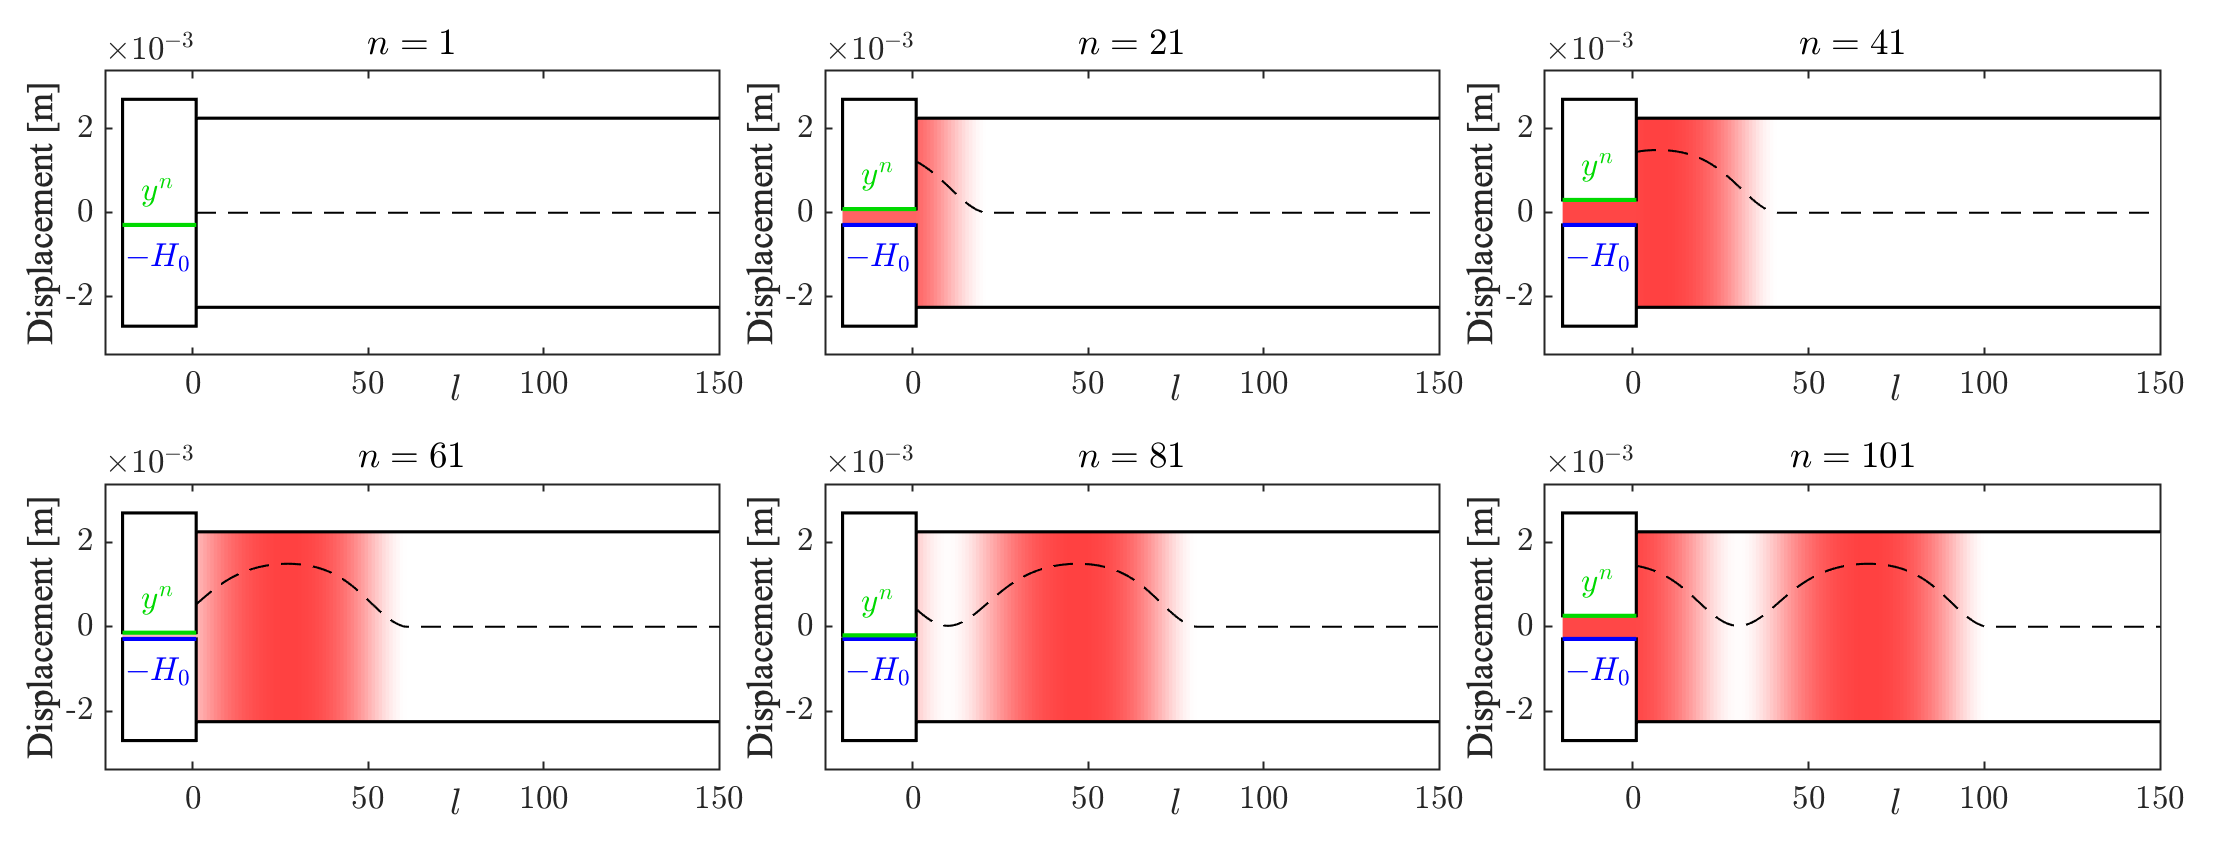
\includegraphics[width=\textwidth]{figures/exciters/lipreed/lipreedImplementation.eps}
    \caption{A lip reed (shown at the left side of the plots) exciting a cylindrical acoustic tube. The y-axis refers to the displacement of the lips and the pressure in the tube $p_l^n$ is shown in red and highlighted with a dashed line (not related to the y-axis).\label{fig:lipreedTube}}
\end{figure}
\section{Energy analysis}\label{sec:energyAnalysisLipreed}
This section performs an energy analysis on the lip reed system, coupled to an acoustic tube using the steps described Section \ref{sec:energyAnalysis}. The analysis follows \cite[Sec 5.1.3, p. 139]{Harrison2018}.

As all physical parameters need to be written out to obtain the correct units, Eq. \eqref{eq:lipReedDimensional} is discretised to get
\begin{equation}\label{eq:discLipreedDimensional}
    M\delta_{tt}y^{\nphSys} = -K\mu_{t\cdot}y^{\nphSys}-R\delta_{t\cdot}y^{\nphSys} + S_\text{r}\Delta p^{\nphSys},
\end{equation} 
and will be used in this analysis. Again, the superscript $n+1/2$ will be suppressed for $y$, $\Delta p$, $U_\text{B}$, $U_\text{r}$, $S_{1/2}$ and $v_{1/2}$ for brevity.

\subsubsection{Step 1: Obtain $\dtp \h$} 
Multiplying Eq. \eqref{eq:discLipreedDimensional} by $(\delta_{t\cdot}y)$, and moving all terms to the left-hand side, yields the rate of change of the energy in the lip reed $\h_\rtxt$:
\begin{equation*}
    \dtp \h_\rtxt = M(\delta_{t\cdot}y^{\nph})(\delta_{tt}y^{\nph}) + K(\delta_{t\cdot}y^{\nph})(\mu_{t\cdot}y^{\nph}) + R(\delta_{t\cdot}y^{\nph})^2 - S_\text{r}(\delta_{t\cdot}y^{\nph})\Delta p^{\nph} = 0.
\end{equation*}
One can substitute Eqs \eqref{eq:Ur}, and \eqref{eq:UbUr} thereafter, to get
\begin{align*}
    \dtp \h_\rtxt = M(\delta_{t\cdot}y^{\nph})(\delta_{tt}y^{\nph}) &+ K(\delta_{t\cdot}y^{\nph})(\mu_{t\cdot}y^{\nph}) + R(\delta_{t\cdot}y^{\nph})^2 \\
    &\quad- \left(\mu_{x-}(S_{1/2}v_{1/2})-U_\text{B}\right)\Delta p^{\nph} = 0.
\end{align*}
Finally, substituting Eq. \eqref{eq:pDiff}, yields
\begin{align*}
    \dtp \h_\rtxt = M(\delta_{t\cdot}y^{\nph})(\delta_{tt}y^{\nph}) &+ K(\delta_{t\cdot}y^{\nph})(\mu_{t\cdot}y^{\nph}) + R(\delta_{t\cdot}y^{\nph})^2 \\
    &\quad+ U_\text{B}\Delta p^{\nph} - \mu_{x-}(S_{1/2}v_{1/2})(P_\mtxt-\mtp p_0^n) = 0.
\end{align*}
One can then include the tube by recalling that $\delta_{t+}\mathfrak{h}_\text{t} = -\mathfrak{b}_\text{r} + \mathfrak{b}_\text{l}$, and that the left boundary term is defined as (Eq. \eqref{eq:firstOrderLeftBoundary})
\begin{equation*}
    \mathfrak{b}_\text{l} = (\mu_{t+}p_0)\mu_{x-}(S_{1/2}v_{1/2}),
\end{equation*} 
and substituting this (ignoring the right boundary term, i.e., $\b_\rtxt = 0$) to get
\begin{align*}
    \dtp (\h_\rtxt +\h_\ttxt) = M(\delta_{t\cdot}y^{\nph})(\delta_{tt}y^{\nph}) &+ K(\delta_{t\cdot}y^{\nph})(\mu_{t\cdot}y^{\nph}) + R(\delta_{t\cdot}y^{\nph})^2 \\
    &\quad+ U_\text{B}\Delta p^{\nph} - \mu_{x-}(S_{1/2}v_{1/2})P_\mtxt = 0.
\end{align*}
\subsubsection{Step 2: Identify energy types and isolate $\dtp$}
Using identities \eqref{eq:prodIdentity1} and \eqref{eq:prodIdentity4}, the energy balance can be shown to be
\begin{equation}\label{eq:powerBalanceLipreed}
    \delta_{t+}\left(\mathfrak{h}_\text{t}+\mathfrak{h}_\text{r}\right) = - \q_\text{r} - \mathfrak{p}_\text{r},
\end{equation}
where the energy of the tube $\h_\ttxt$ is as defined in Eq. \eqref{eq:energyBalanceFirstOrder} and the energy of the mass is
\begin{equation}
    \h_\rtxt = \t_\rtxt + \v_\rtxt, \qwiq \t_\rtxt = \frac{M}{2}(\delta_{t-}y)^2, \qaq \v = \frac{K}{2}\mu_{t-}(y^2).
\end{equation}
Furthermore, the damping term is defined as
\begin{equation}
    \mathfrak{q}_\text{r} = R(\dtd y)^2 + U_\text{B}\Delta p^{\nph},
\end{equation}
and the input power as
\begin{equation}
    \mathfrak{p}_\text{r} = -(U_\text{B} + U_\text{r})P_\text{m}.
\end{equation}
It is interesting to note that due to the choice of discretisation of the lip reed, $\t_\rtxt$, $\v_\rtxt$ and $\q_\rtxt$ are non-negative, making the lip reed strictly dissipative and thus inherently stable. 

\subsubsection{Step 3: Check units}
The kinetic and potential energy of the lip reed can be written in their units as
\begin{align*}
    \t_\rtxt = \frac{M}{2}(\delta_{t-}y)^2 &\ \overset{\text{in units}}{\xrightarrow{\hspace*{1cm}}} \quad\text{kg}\cdot(\text{s}^{-1}\cdot \text{m})^{2}= \text{kg}\cdot\text{m}^2\cdot\text{s}^{-2},\\
    \v_\rtxt = \frac{K}{2}\mu_{t-}(y^2)&\ \overset{\text{in units}}{\xrightarrow{\hspace*{1cm}}} \quad \text{N} \cdot \text{m}^{-1} \cdot \text{m}^2 = \text{kg}\cdot\text{m}^2\cdot\text{s}^{-2},
\end{align*}
and have the correct units. Recalling that the damping and input power terms need to have units of kg$\cdot$ m$^2 \cdot $s$^{-3}$, writing the individual components of these terms in their respective units, yields
\begin{align*}
    R(\dtd y)^2 &\ \overset{\text{in units}}{\xrightarrow{\hspace*{1cm}}} \quad\text{kg}\cdot\text{s}^{-1}\cdot(\text{s}^{-1}\cdot \text{m})^{2} = \text{kg} \cdot \text{m}^2 \cdot \text{s}^{-3} ,\\
    U_\text{B}\Delta p^{\nph}&\ \overset{\text{in units}}{\xrightarrow{\hspace*{1cm}}} \quad \text{m}^3 \cdot \text{s}^{-1}\cdot \text{kg}\cdot \text{m}^{-1}\cdot \text{s}^{-2}= \text{kg} \cdot \text{m}^2 \cdot \text{s}^{-3},\\
    -(U_\Btxt + U_\rtxt)P_\mtxt&\ \overset{\text{in units}}{\xrightarrow{\hspace*{1cm}}} \quad \text{m}^3 \cdot \text{s}^{-1}\cdot \text{kg}\cdot \text{m}^{-1}\cdot \text{s}^{-2}= \text{kg} \cdot \text{m}^2 \cdot \text{s}^{-3},
\end{align*}
and shows that the units are indeed correct.
\subsubsection{Step 4: Implementation}
Figure \ref{fig:lipReedEnergy} shows the energetic output of the lip reed coupled to an acoustic tube, corresponding to the behaviour shown in Figure \ref{fig:lipreedTube}. The total energy of the system increases due to the input pressure and is mainly transferred to the tube. That the lip reed is oscillating can be observed from the oscillations in its kinetic and potential energy. The normalised energy (using Eq. \eqref{eq:normalisedEnergyDamping}) does not include the first time index, as one full iteration of the coupling is necessary to yield a correct energy calculation. Instead, one starts at $n=1$ and uses $\h^1$ instead of $\h^0$ in Eq. \eqref{eq:normalisedEnergyDamping}.

\begin{figure}[h]
    \centering
    \begin{tikzpicture}[->,node distance=3cm,
        thick,main node/.style={circle,draw}]
    
        \node[] (image) at (0,0) {
        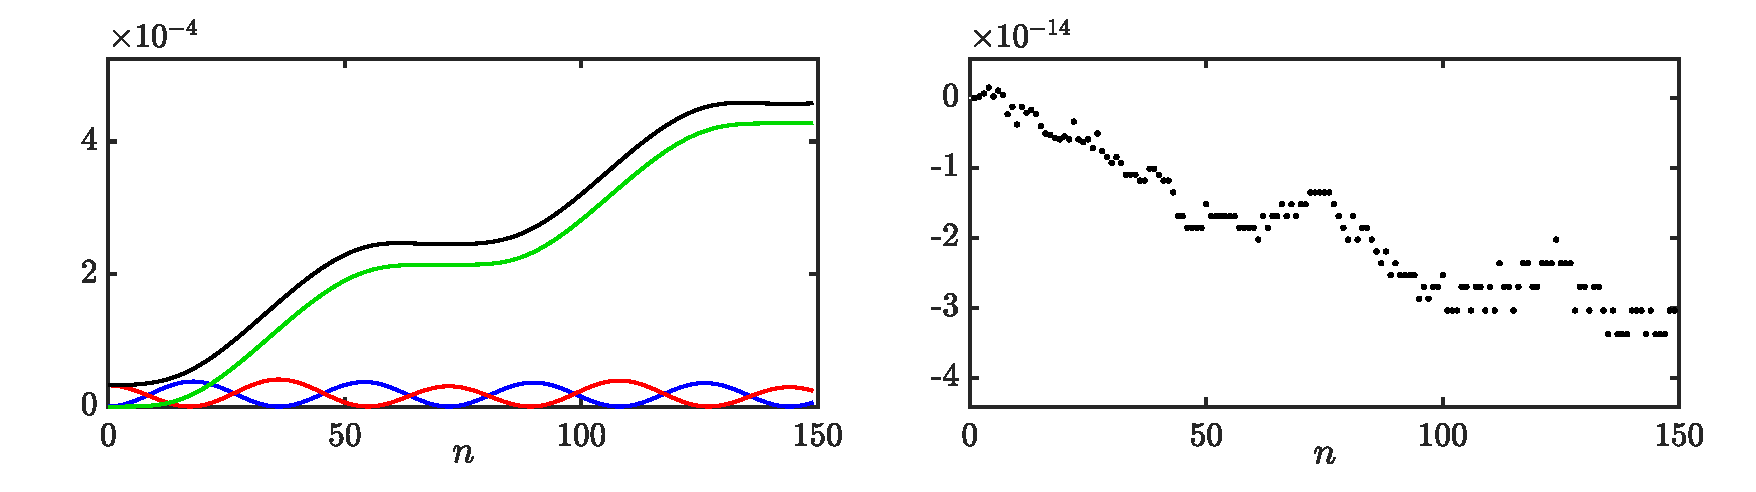
\includegraphics[width=\textwidth]{figures/exciters/lipreed/lipreedEnergy.eps}
        };
    
        \node[] (he) at (0.2,0.5) {\small $\mathfrak{h}_\text{e}$};

        \node[] (h) at (-5.8, 1) {\small $\mathfrak{h}$};
        \node[] (v) at (-5.8, 0.5) {\small $\color[HTML]{00DB00}\mathfrak{h}_\ttxt$};
        \node[] (t) at (-5.8, 0) {\small $\color{red}\mathfrak{v}_\rtxt$};
        \node[] (c) at (-5.8, -0.5) {\small $\color{blue}\mathfrak{t}_\rtxt$};

      \end{tikzpicture}
      \caption{The energy of the acoustic tube (green), the potential energy (red) the kinetic energy of the lip reed (blue), and the total energy (black) of the system corresponding to Figure \ref{fig:lipreedTube}. The right panel shows the normalised energy (according to Eq. \eqref{eq:normalisedEnergyDamping}, starting at $n=1$) and shows that the deviation of the energy is within machine precision. \label{fig:lipReedEnergy}}
\end{figure}
